\documentclass[11pt]{article}

\usepackage[margin=1in]{geometry}
\usepackage[T1]{fontenc}
\usepackage{lmodern}
\usepackage{microtype}
\usepackage{graphicx}
\usepackage{booktabs}
\usepackage{longtable}
\usepackage{array}
\usepackage{caption}
\usepackage{subcaption}
\usepackage{xcolor}
\usepackage{hyperref}
\usepackage[authoryear,round]{natbib}
\usepackage{float}
\usepackage{placeins}
\usepackage{enumitem}
\usepackage{listings}
\usepackage{tikz}
\usetikzlibrary{arrows.meta,positioning,shapes.geometric,calc}

\hypersetup{
  colorlinks=true,
  linkcolor=blue,
  urlcolor=blue,
  citecolor=blue
}

% --- Rust listings (minimal, no external deps) ---
\lstdefinelanguage{Rust}{
  keywords={as, break, const, continue, crate, else, enum, extern, false, fn, for, if, impl, in, let, loop, match, mod, move, mut, pub, ref, return, self, Self, static, struct, super, trait, true, type, unsafe, use, where, while, async, await, dyn},
  sensitive=true,
  comment=[l]{//},
  morecomment=[s]{/*}{*/},
  morestring=[b]",
}

\lstset{
  language=Rust,
  basicstyle=\ttfamily\small,
  columns=fullflexible,
  keepspaces=true,
  frame=single,
  breaklines=true,
  showstringspaces=false,
  keywordstyle=\bfseries\color{blue!60!black},
  commentstyle=\color{green!40!black},
  stringstyle=\color{red!60!black}
}

\title{Medical Care Robot Coordination System (MCRoCS, ``McRocks''): Written Report}
\author{FA, Haochen\\Student ID: 24113347D\\COMP2432 Operating Systems}
\date{25/26 Sem 2}

\begin{document}
\maketitle

\begin{abstract}
Medical Care Robot Coordination System (MCRoCS, ``McRocks'') is a lightweight operating-system core for coordinating multiple medical-care robots with safe concurrency. The system implements exactly three required services: a thread-safe task queue, exclusive zone access control, and a heartbeat-based health monitor. The main challenges were avoiding race conditions while keeping critical sections small and ensuring that offline detection was observable in a short demo. The solution uses Rust's \texttt{Mutex} and \texttt{Condvar} to serialize access to shared state, plus atomics for lightweight counters inside the simulation \citep{rustmutex,rustcondvar}. A CLI-driven demo shows multiple robots fetching tasks concurrently, entering zones without overlap, and a robot timing out after it stops heartbeats. Benchmarks and stress sweeps report throughput, zone wait times, and CPU usage, while tests validate single-consumer task behavior, zone exclusivity, and timeout detection. The result is a minimal, correct coordination layer aligned with the project's OS learning outcomes and refined to reduce benchmark overhead without expanding the project's scope.
\end{abstract}

\section{Introduction}
Modern hospitals increasingly rely on autonomous robots for delivery, sanitation, and assistance. In such settings, coordination errors are not merely inconveniences; they can cause safety incidents, resource contention, or service delays. Medical Care Robot Coordination System addresses this by building a minimal operating-system core that enforces safe concurrency without introducing complex scheduling or preemption. The goal is not to model a complete robot control stack but to implement and demonstrate three essential coordination services under concurrent load: a task queue that ensures each task is assigned at most once, a zone access controller that prevents two robots from occupying the same physical zone simultaneously, and a health monitor that detects robots that stop sending heartbeats.

The project objectives are closely tied to operating-systems fundamentals. First, it must implement correct concurrency control so that shared state remains consistent under multiple threads. Second, it must use explicit synchronization to prevent race conditions. Third, it must coordinate the interactions among threads to produce a predictable, observable outcome that can be demonstrated in a short runtime. The minimal scope is intentional: by removing preemption and complex scheduling policies, the design keeps focus on safety invariants and synchronization correctness. This also makes it possible to reason about system state transitions and to write tests that are both meaningful and deterministic.

The implementation is a Rust Cargo project organized around three core modules, plus a simulation driver. Each component uses safe synchronization primitives (\texttt{Mutex}, \texttt{Condvar}, and atomics) and follows a narrow-lock-scope design to minimize contention and avoid deadlocks. Rust's ownership model and standard library concurrency support help enforce data-race freedom by construction \citep{klabnik2022}. The simulation spawns multiple robot threads, drives task consumption, enforces zone ownership, and checks for offline robots in both deterministic demo mode and benchmark/stress offline mode. The command-line interface supports a default demo as well as benchmark and stress modes that print human-readable summaries and tables for analysis. This report details the design, implementation, and evaluation of the project and connects the observed behaviors to OS-level concurrency concepts.

\section{Related Works}
Concurrency control has been a central operating-systems concern since early multiprogramming. Seminal work on mutual exclusion and synchronization, including Dijkstra's and Lamport's classic algorithms, established the need for explicit coordination when multiple execution contexts share resources \citep{dijkstra1965,lamport1978}. Practical guidance on programming with threads reinforced these principles for real systems \citep{birrell1989}. Monitors and condition variables, popularized in systems like Mesa, formalized a practical pattern: a shared state protected by a lock, with threads waiting on conditions that are re-checked after waking \citep{hoare1974,lampson1980}. MCRoCS uses this pattern directly, with \texttt{Mutex}-guarded state and \texttt{Condvar} waits for both task queues and zone access \citep{rustmutex,rustcondvar}. This mirrors the approach described in modern OS texts that emphasize correct locking, short critical sections, and explicit wait conditions \citep{arpaci2018,silberschatz2018,tanenbaum2015}.

Task queues are a common concurrency primitive in systems software, appearing in thread pools, work-stealing schedulers, and I/O dispatch loops \citep{arpaci2018,silberschatz2018}. In many high-performance systems, lock-free or multi-queue designs reduce contention, but they are more complex to reason about \citep{herlihy2020}. For the project, the requirement is correctness and clarity rather than maximum throughput. A single FIFO queue guarded by a mutex and condition variable provides strong safety properties: tasks are consumed at most once, and consumers can block efficiently until work arrives \citep{hoare1974}. This is consistent with the ``producer-consumer'' model in classical synchronization literature and is a well-understood pattern for teaching concurrency \citep{downey2016}. Modern practitioner-focused texts likewise emphasize explicit synchronization for shared state in concurrent programs \citep{williams2019}.

Resource coordination often reduces to mutual exclusion on a namespace of shared resources \citep{silberschatz2018,tanenbaum2015}. The zone controller in the project is conceptually similar to a lock table or resource allocator: each zone has at most one owner at a time \citep{gray1993}. This resembles database lock managers and OS-level resource maps where ownership must be unambiguous. In the current implementation, the configured zones are stored in a fixed, direct-indexed slot table, which keeps ownership explicit while avoiding map lookups on the hot path. The use of a condition variable to wait for zone availability aligns with monitor-based coordination patterns \citep{hoare1974,lampson1980}. It is also consistent with the trade-offs discussed in modern concurrency references: coarse-grained locking simplifies correctness reasoning but can limit parallelism if the lock is held too long \citep{herlihy2020}. In the project, each zone acquisition holds the lock only long enough to check and update the ownership slot, minimizing contention.

Health monitoring through heartbeats is common in distributed systems and fault-tolerant designs \citep{lynch1996,chandra1996}. In such systems, nodes periodically emit a signal that a watcher uses to infer liveness. Failure detection is imperfect and depends on timeout selection; shorter timeouts detect failures faster but increase false positives \citep{lynch1996}. The project adopts a simple timeout-based scheme suitable for a single-process simulation. The monitor maintains a last-seen timestamp per robot and marks robots offline once their heartbeat exceeds a configured duration. This is consistent with classic failure detector models and highlights the OS-level idea of watchdog timers \citep{chandra1996}.

Compared with more sophisticated approaches---such as lock-free queues, adaptive timeouts, or priority-aware scheduling---the project intentionally chooses minimal mechanisms. This aligns with the project's pedagogical goals: by using straightforward, well-documented primitives, it becomes easier to explain the safety invariants and to provide testable evidence of correctness. The design therefore emphasizes clarity and correctness over performance, while still enabling quantitative benchmarking.

\section{Implementation}
\subsection{Architecture overview}
MCRoCS is organized around a CLI entry point and three execution modes (demo, benchmark, stress). The core modules implement task queueing, zone access control, and health monitoring. The simulation driver (\texttt{sim.rs}) wires these components, spawns worker threads, and collects metrics. Logging is gated to debug builds, while release mode keeps output concise for measurement and grading.

\begin{figure}[H]
  \centering
  \resizebox{\linewidth}{!}{%
  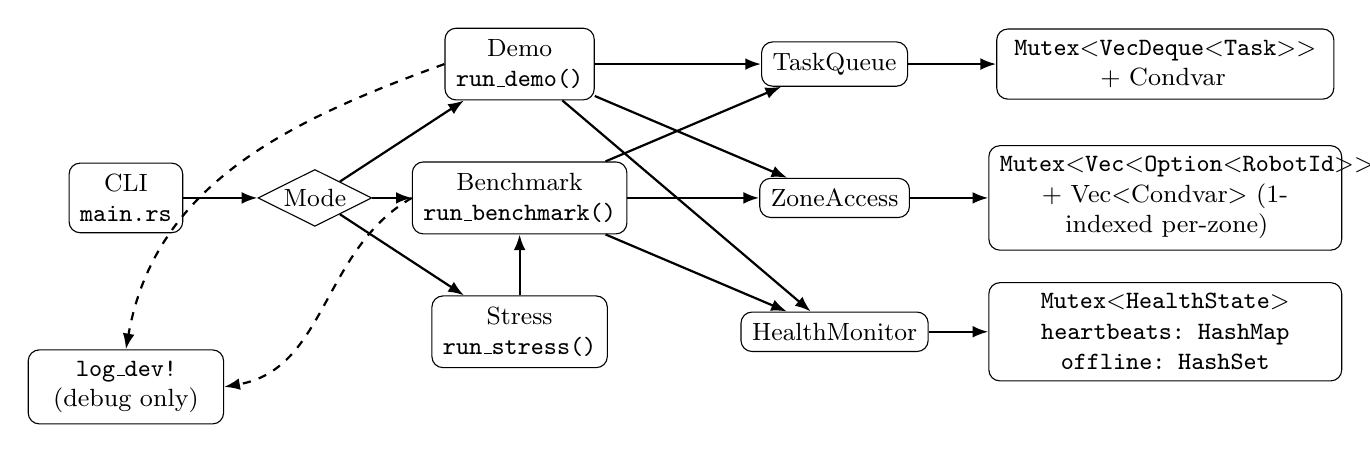
\begin{tikzpicture}[
    box/.style={draw, rounded corners, align=center, inner sep=4pt, font=\small},
    decision/.style={draw, diamond, aspect=2.0, align=center, inner sep=1pt, font=\small},
    arr/.style={-{Latex[length=2mm]}, thick},
    darr/.style={-{Latex[length=2mm]}, thick, dashed}
  ]
    % Entry and routing
    \node[box] (cli) at (0,0) {CLI\\\texttt{main.rs}};
    \node[decision] (mode) at (2.4,0) {Mode};
    \node[box] (demo)   at (5.0,  1.7) {Demo\\\texttt{run\_demo()}};
    \node[box] (bench)  at (5.0,  0.0) {Benchmark\\\texttt{run\_benchmark()}};
    \node[box] (stress) at (5.0, -1.7) {Stress\\\texttt{run\_stress()}};
    \node[box, text width=22mm] (log) at (0, -2.4) {\texttt{log\_dev!}\\(debug only)};

    % Three separate service nodes
    \node[box] (tq) at (9.0,  1.7) {TaskQueue};
    \node[box] (za) at (9.0,  0.0) {ZoneAccess};
    \node[box] (hm) at (9.0, -1.7) {HealthMonitor};

    % Sync-detail nodes (one per service)
    \node[box, text width=40mm] (tqsync) at (13.2,  1.7)
      {\texttt{Mutex\textless VecDeque\textless Task\textgreater\textgreater}\\+ Condvar};
    \node[box, text width=42mm] (zasync) at (13.2,  0.0)
      {\texttt{Mutex\textless Vec\textless Option\textless RobotId\textgreater\textgreater\textgreater}\\+ Vec\textless Condvar\textgreater\ (1-indexed per-zone)};
    \node[box, text width=42mm] (hmsync) at (13.2, -1.7)
      {\texttt{Mutex\textless HealthState\textgreater}\\\texttt{heartbeats: HashMap}\\\texttt{offline: HashSet}};

    % Routing arrows
    \draw[arr] (cli)  -- (mode);
    \draw[arr] (mode) -- (demo);
    \draw[arr] (mode) -- (bench);
    \draw[arr] (mode) -- (stress);
    \draw[arr] (stress) -- (bench);

    % Demo → each service
    \draw[arr] (demo) -- (tq);
    \draw[arr] (demo) -- (za);
    \draw[arr] (demo) -- (hm);

    % Bench → each service
    \draw[arr] (bench) -- (tq);
    \draw[arr] (bench) -- (za);
    \draw[arr] (bench) -- (hm);

    % Service → sync detail
    \draw[arr] (tq) -- (tqsync);
    \draw[arr] (za) -- (zasync);
    \draw[arr] (hm) -- (hmsync);

    % Debug-only log coupling (dashed)
    \draw[darr] (demo.west)  to[out=200, in=80]  (log.north);
    \draw[darr] (bench.west) to[out=210, in=10]  (log.east);
  \end{tikzpicture}
  }
  \caption{Architecture overview: CLI routes to execution mode; \texttt{run\_demo()} and \texttt{run\_benchmark()} each use all three core services independently. \texttt{run\_stress()} delegates to \texttt{run\_benchmark()}. Each service has its own synchronization primitive (shown at right). Dashed arrows indicate debug-only coupling (\texttt{log\_dev!} is a no-op in release builds). The zone controller uses direct-indexed per-zone state, and the health monitor keeps heartbeat and offline state under one mutex.}
  \label{fig:architecture}
\end{figure}

\subsection{Task queue}
The task queue uses a \texttt{Mutex<\allowbreak VecDeque<\allowbreak Task>>} to serialize access to an internal FIFO, and a \texttt{Condvar} to block consumers when the queue is empty \citep{rustmutex,rustcondvar}. This design ensures that each task is consumed at most once, and it prevents busy waiting. The critical section is minimal: a consumer holds the lock only long enough to check for a task and pop it. When the queue is empty, the thread waits on the condition variable, which releases the lock and re-acquires it on wake.

\noindent\textbf{Critical code path (blocking pop):}
\begin{lstlisting}
pub fn pop_blocking_or_closed(&self) -> Option<Task> {
    let mut guard = self.inner.lock().expect("task queue mutex poisoned");
    loop {
        if let Some(task) = guard.queue.pop_front() {
            return Some(task);
        }
        if guard.closed {
            return None;
        }
        guard = self.available.wait(guard).expect("condvar wait failed");
    }
}
\end{lstlisting}

\begin{figure}[H]
  \centering
  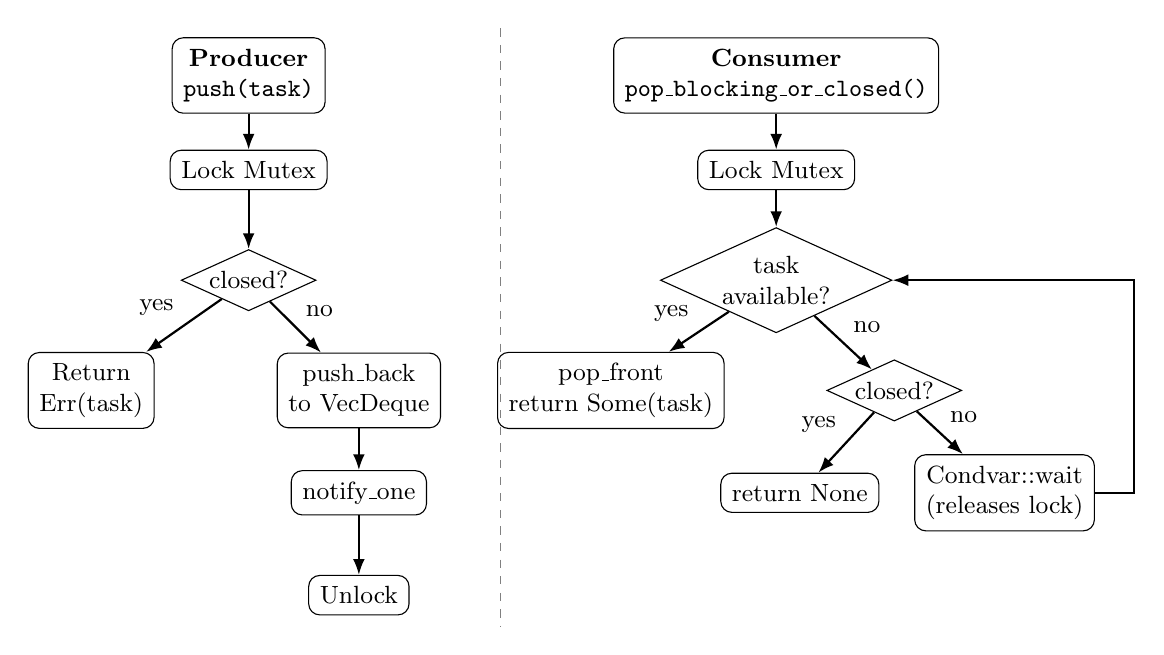
\begin{tikzpicture}[
    node distance=7mm and 10mm,
    box/.style={draw, rounded corners, align=center, inner sep=4pt, font=\small},
    decision/.style={draw, diamond, aspect=2.2, align=center, inner sep=1pt, font=\small},
    arr/.style={-{Latex[length=2mm]}, thick}
  ]
    %% ---- Left column: Producer (push) ----
    \node[box] (p0) at (-3.2, 0)    {\textbf{Producer}\\\texttt{push(task)}};
    \node[box] (p1) at (-3.2,-1.2)  {Lock Mutex};
    \node[decision] (p2) at (-3.2,-2.6) {closed?};
    \node[box] (p3) at (-5.2,-4.0)  {Return\\Err(task)};
    \node[box] (p4) at (-1.8,-4.0)  {push\_back\\to VecDeque};
    \node[box] (p5) at (-1.8,-5.3)  {notify\_one};
    \node[box] (p6) at (-1.8,-6.6)  {Unlock};

    \draw[arr] (p0) -- (p1);
    \draw[arr] (p1) -- (p2);
    \draw[arr] (p2) -- node[above left, font=\small]{yes} (p3);
    \draw[arr] (p2) -- node[above right, font=\small]{no}  (p4);
    \draw[arr] (p4) -- (p5);
    \draw[arr] (p5) -- (p6);

    %% ---- Right column: Consumer (pop_blocking_or_closed) ----
    \node[box] (c0) at (3.5, 0)    {\textbf{Consumer}\\\texttt{pop\_blocking\_or\_closed()}};
    \node[box] (c1) at (3.5,-1.2)  {Lock Mutex};
    \node[decision] (c2) at (3.5,-2.6) {task\\available?};
    \node[box] (c3) at (1.4,-4.0)  {pop\_front\\return Some(task)};
    \node[decision] (c4) at (5.0,-4.0) {closed?};
    \node[box] (c5) at (3.8,-5.3)  {return None};
    \node[box] (c6) at (6.4,-5.3)  {Condvar::wait\\(releases lock)};

    \draw[arr] (c0) -- (c1);
    \draw[arr] (c1) -- (c2);
    \draw[arr] (c2) -- node[above left, font=\small]{yes} (c3);
    \draw[arr] (c2) -- node[above right, font=\small]{no}  (c4);
    \draw[arr] (c4) -- node[above left, font=\small]{yes}  (c5);
    \draw[arr] (c4) -- node[above right, font=\small]{no}  (c6);
    % wait loops back to the task-available check
    \draw[arr] (c6.east) -- ++(0.5,0) |- (c2.east);

    %% ---- Vertical separator ----
    \draw[dashed, gray] (0, 0.6) -- (0, -7.0);
  \end{tikzpicture}
  \caption{TaskQueue producer and consumer paths: \texttt{push} notifies one consumer; blocking \texttt{pop\_blocking\_or\_closed} waits until a task arrives or the queue closes.}
  \label{fig:tq-flow}
\end{figure}

The queue also supports \texttt{try\_pop} for non-blocking access and a \texttt{close} operation that wakes all blocked consumers. Tests validate that tasks are consumed exactly once across multiple threads, that blocking consumers wake on push, and that closure unblocks waiting threads. These tests directly target the invariants required by the project: single assignment of tasks and safe concurrent access.

\subsection{Zone access control}
The zone controller enforces exclusive occupancy per zone using a \texttt{Mutex<Vec<Option<RobotId>>>} and a vector of per-zone \texttt{Condvar}s \citep{rustmutex,rustcondvar}. Zones are 1-indexed and validated against the configured zone count, so each zone maps directly to one ownership slot and one condvar. This keeps the representation simple and removes hash-map lookup overhead from the hot path while preserving the same mutual-exclusion behavior. When a zone becomes available, the owner calls \texttt{notify\_one} on that zone's condvar, waking exactly one contender rather than all waiters.

\noindent\textbf{Critical code path (acquire):}
\begin{lstlisting}
pub fn acquire(&self, zone: ZoneId, robot: RobotId) {
    let idx = self.zone_index(zone);
    let mut guard = self.occupied.lock().expect("zone mutex poisoned");
    loop {
        if guard[idx].is_none() {
            guard[idx] = Some(robot);
            return;
        }
        guard = self.condvars[idx].wait(guard).expect("condvar wait failed");
    }
}
\end{lstlisting}

This approach keeps the lock scope short and avoids deadlocks because only one lock is held at a time. Per-zone condvars eliminate unnecessary wakeups when zones are independent, reducing contention under high concurrency. The design is intentionally conservative: it prioritizes correctness and explicit ownership tracking. Unit tests spawn multiple contenders for a single zone and verify that the observed occupancy never exceeds one; additional tests check that the occupied-zone snapshot matches current ownership and that out-of-range zones are rejected in debug builds. In release builds, non-owner release attempts are logged and rejected, preserving safety even without debug assertions.

\begin{figure}[H]
  \centering
  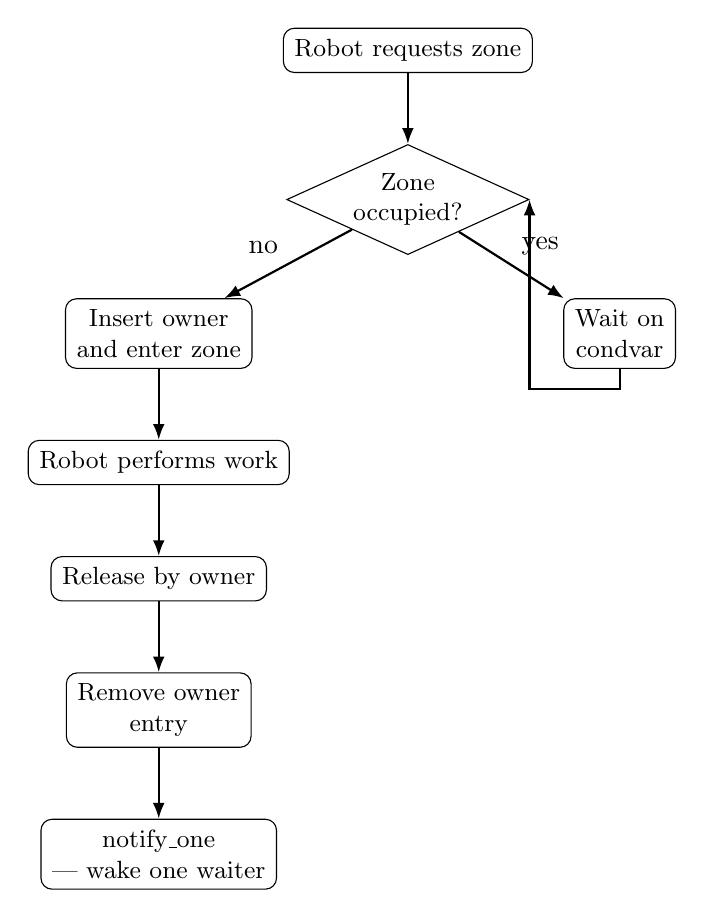
\begin{tikzpicture}[
    node distance=9mm and 12mm,
    box/.style={draw, rounded corners, align=center, inner sep=4pt, font=\small},
    decision/.style={draw, diamond, aspect=2.2, align=center, inner sep=1pt, font=\small},
    arr/.style={-{Latex[length=2mm]}, thick}
  ]
    \node[box] (a) {Robot requests zone};
    \node[decision, below=of a] (b) {Zone\\occupied?};
    \node[box, below left=of b] (c) {Insert owner\\and enter zone};
    \node[box, below right=of b] (d) {Wait on\\condvar};
    \node[box, below=of c] (e) {Robot performs work};
    \node[box, below=of e] (f) {Release by owner};
    \node[box, below=of f] (g) {Remove owner\\entry};
    \node[box, below=of g] (h) {notify\_one\\--- wake one waiter};

    \draw[arr] (a) -- (b);
    \draw[arr] (b) -- node[above left]{no} (c);
    \draw[arr] (b) -- node[above right]{yes} (d);
    \draw[arr] (d) -- ++(0,-7mm) -| (b.east);
    \draw[arr] (c) -- (e);
    \draw[arr] (e) -- (f);
    \draw[arr] (f) -- (g);
    \draw[arr] (g) -- (h);
  \end{tikzpicture}
  \caption{Zone access control logic (TikZ adaptation of the implementation flow).}
  \label{fig:zone-flow}
\end{figure}

\subsection{Health monitor}
The health monitor uses a single-lock design: a \texttt{Mutex<HealthState>} that contains both a \texttt{HashMap<RobotId, Instant>} for heartbeat timestamps and a \texttt{HashSet<RobotId>} for the offline set \citep{rustmutex}. This keeps heartbeat updates and offline detection inside one coherent critical section and removes the need for cross-lock coordination. The implementation relies on monotonic timestamps for timeout comparison \citep{rustinstant}.

\noindent\textbf{Critical code path (offline detection):}
\begin{lstlisting}
pub fn detect_offline(&self, timeout: Duration) -> HashSet<RobotId> {
    let now = Instant::now();
    let mut guard = self.inner.lock().expect("health monitor mutex poisoned");
    let overdue: Vec<_> = guard
        .heartbeats
        .iter()
        .filter_map(|(&robot, &last)| {
            if now.duration_since(last) > timeout { Some(robot) } else { None }
        })
        .collect();
    for robot in overdue {
        guard.offline.insert(robot);
    }
    guard.offline.clone()
}
\end{lstlisting}

\begin{figure}[H]
  \centering
  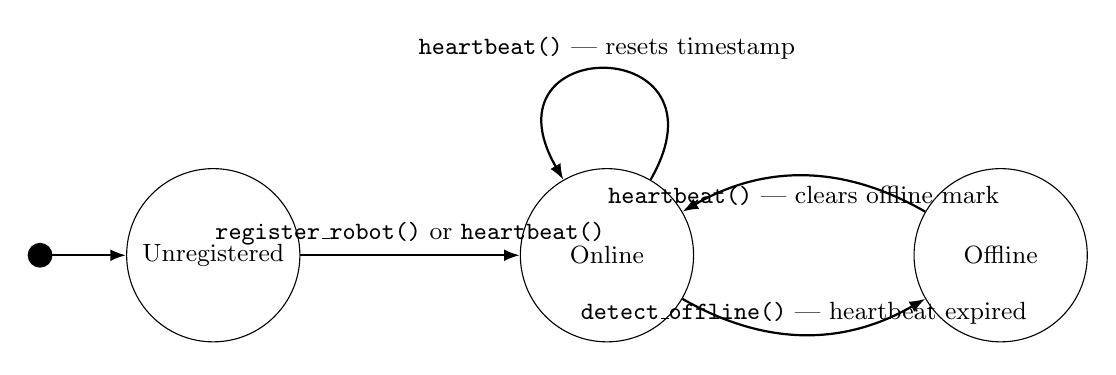
\begin{tikzpicture}[
    state/.style={draw, circle, minimum size=22mm, align=center, font=\small},
    arr/.style={-{Latex[length=2mm]}, thick}
  ]
    % States
    \node[state] (unreg)   at (0,   0)  {Unregistered};
    \node[state] (online)  at (5.0, 0)  {Online};
    \node[state] (offline) at (10.0, 0) {Offline};

    % Initial pseudo-state
    \node[draw, fill, circle, minimum size=3mm, inner sep=0pt] (init) at (-2.2, 0) {};
    \draw[arr] (init) -- (unreg);

    % Unregistered → Online
    \draw[arr] (unreg) -- node[above, font=\small]
      {\texttt{register\_robot()} or \texttt{heartbeat()}} (online);

    % Online self-loop (top)
    \draw[arr] (online) to[out=60, in=120, looseness=5]
      node[above, font=\small] {\texttt{heartbeat()} — resets timestamp} (online);

    % Online → Offline
    \draw[arr] (online) to[out=-30, in=210]
      node[above, font=\small] {\texttt{detect\_offline()} — heartbeat expired}
      (offline);

    % Offline → Online
    \draw[arr] (offline) to[out=150, in=30]
      node[below, font=\small] {\texttt{heartbeat()} — clears offline mark}
      (online);
  \end{tikzpicture}
  \caption{HealthMonitor robot state transitions. A robot enters \textit{Online} on first heartbeat, transitions to \textit{Offline} when \texttt{detect\_offline()} finds its timestamp overdue, and recovers to \textit{Online} on the next heartbeat.}
  \label{fig:hm-states}
\end{figure}

Tests ensure that robots are marked offline after timeouts and that a new heartbeat clears the offline status. A test-only hook allows deterministic verification without sleeping, preventing flaky test behavior.

\subsection{Simulation and CLI}

\begin{figure}[H]
  \centering
  \resizebox{0.97\linewidth}{!}{%
  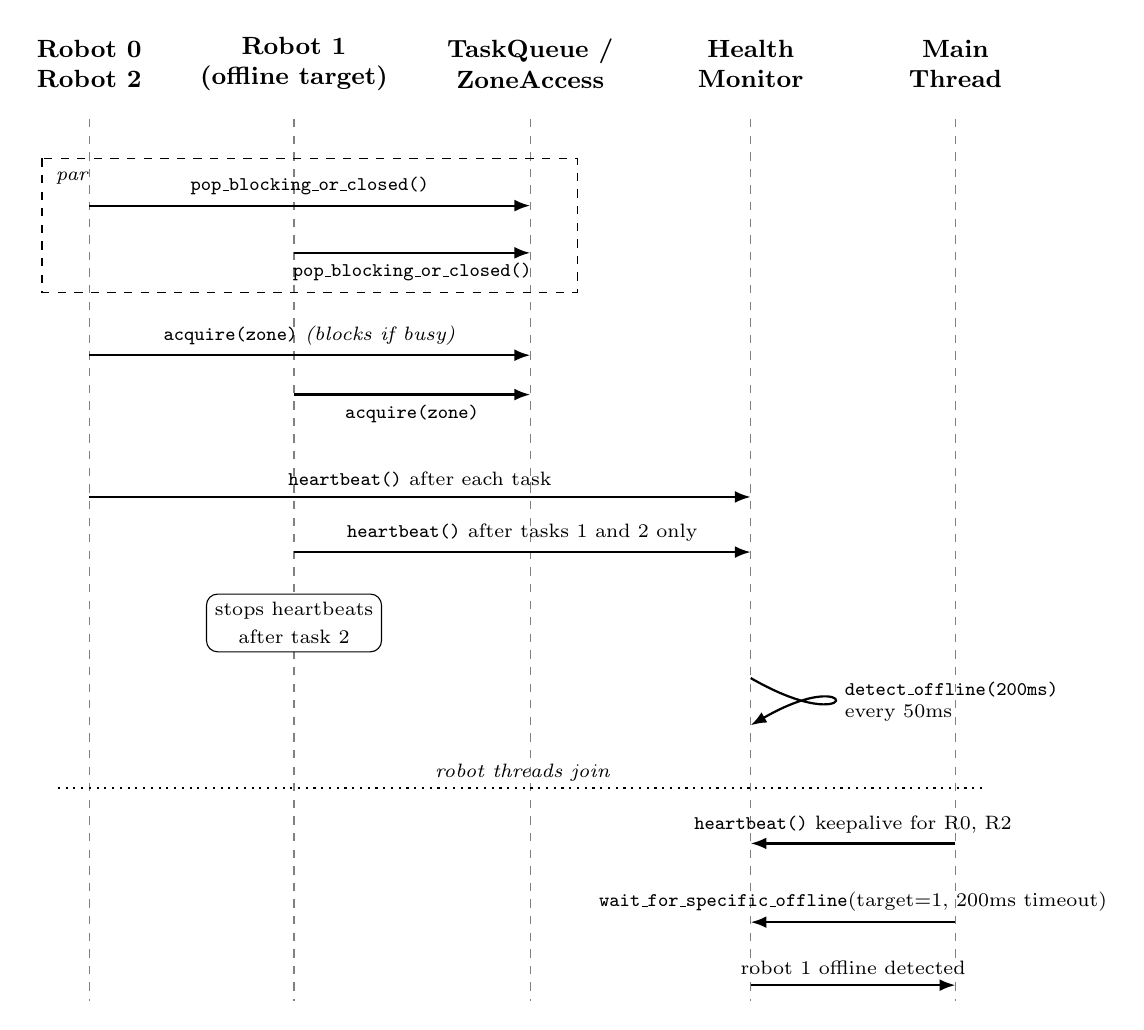
\begin{tikzpicture}[
    arr/.style={-{Latex[length=2mm]}, thick},
    note/.style={draw, rounded corners, align=center, inner sep=3pt, font=\small, fill=white},
    tl/.style={dashed, gray}
  ]
    % Participant headers
    \node[font=\small\bfseries, align=center] at (0,    0.7) {Robot 0\\Robot 2};
    \node[font=\small\bfseries, align=center] at (2.6,  0.7) {Robot 1\\(offline target)};
    \node[font=\small\bfseries, align=center] at (5.6,  0.7) {TaskQueue /\\ZoneAccess};
    \node[font=\small\bfseries, align=center] at (8.4,  0.7) {Health\\Monitor};
    \node[font=\small\bfseries, align=center] at (11.0, 0.7) {Main\\Thread};

    % Timelines
    \draw[tl] (0,    0) -- (0,    -11.2);
    \draw[tl] (2.6,  0) -- (2.6,  -11.2);
    \draw[tl] (5.6,  0) -- (5.6,  -11.2);
    \draw[tl] (8.4,  0) -- (8.4,  -11.2);
    \draw[tl] (11.0, 0) -- (11.0, -11.2);

    % par block bracket
    \draw[dashed, thin] (-0.6, -0.5) rectangle (6.2, -2.2);
    \node[font=\scriptsize\itshape, anchor=north west] at (-0.55, -0.55) {par};

    % 1. Concurrent pop_blocking_or_closed
    \draw[arr] (0,   -1.1) -- node[above, font=\scriptsize] {\texttt{pop\_blocking\_or\_closed()}} (5.6, -1.1);
    \draw[arr] (2.6, -1.7) -- node[below, font=\scriptsize] {\texttt{pop\_blocking\_or\_closed()}} (5.6, -1.7);

    % 2. acquire(zone)
    \draw[arr] (0,   -3.0) -- node[above, font=\scriptsize] {\texttt{acquire(zone)} \textit{(blocks if busy)}} (5.6, -3.0);
    \draw[arr] (2.6, -3.5) -- node[below, font=\scriptsize] {\texttt{acquire(zone)}} (5.6, -3.5);

    % 3. R0/R2 heartbeat after each task
    \draw[arr] (0,   -4.8) -- node[above, font=\scriptsize] {\texttt{heartbeat()} after each task} (8.4, -4.8);

    % 4. R1 heartbeat — tasks 1 and 2 only
    \draw[arr] (2.6, -5.5) -- node[above, font=\scriptsize] {\texttt{heartbeat()} after tasks 1 and 2 only} (8.4, -5.5);

    % 5. R1 stops heartbeats note
    \node[note] at (2.6, -6.4) {\scriptsize stops heartbeats\\[-1pt]\scriptsize after task 2};

    % 6. detect_offline self-call on HM (right-side loop)
    \draw[arr] (8.4, -7.1) to[out=-30, in=30, looseness=7]
      node[right, font=\scriptsize, align=left] {\texttt{detect\_offline(200ms)}\\every 50ms} (8.4, -7.7);

    % Divider: robot threads join
    \draw[dotted, thick] (-0.4, -8.5) -- (11.4, -8.5);
    \node[font=\scriptsize\itshape] at (5.5, -8.3) {robot threads join};

    % 7. Main keepalive heartbeats for R0, R2
    \draw[arr] (11.0, -9.2) -- node[above, font=\scriptsize] {\texttt{heartbeat()} keepalive for R0, R2} (8.4, -9.2);

    % 8. wait_for_specific_offline
    \draw[arr] (11.0, -10.2) -- node[above, font=\scriptsize]
      {\texttt{wait\_for\_specific\_offline}(target=1, 200ms timeout)} (8.4, -10.2);

    % 9. HM → Main: offline detected
    \draw[arr] (8.4, -11.0) -- node[above, font=\scriptsize] {robot 1 offline detected} (11.0, -11.0);

  \end{tikzpicture}
  }
  \caption{Demo sequence: robots concurrently fetch tasks and acquire zones; Robot 1 stops heartbeats after task 2, triggering offline detection.}
  \label{fig:robot-sequence}
\end{figure}

The CLI (\texttt{main.rs}) provides three entry points: demo, benchmark, and stress. In demo mode, robot 1 is the deterministic offline target: it stops heartbeats mid-run while non-target robots are kept alive during final timeout verification. The summary reports \texttt{offline\_target}, \texttt{detected}, per-robot task counts, and zone-safety fields. Shared ownership of core services uses reference-counted pointers \citep{rustarc}.

Benchmarks and stress runs reuse the same core logic and report elapsed time, throughput, average zone wait, CPU usage (when available), and validation flags (duplicate tasks, zone violations). In offline benchmark/stress mode, the system waits for any offline detection after workload completion, so the final offline count may exceed one depending on timing. In normal benchmark/stress mode, the background health-monitor thread is not spawned, which avoids paying offline-detection overhead when liveness is not part of the measured scenario. These runs are tuned for repeatable, observable output rather than realism.

From an implementation perspective, the CLI also enforces strict input validation to keep experiments reproducible. Invalid values (for example zero robots or zero zones) are rejected with a clear usage message, and stress lists can preserve defaults through explicit placeholders. This reduces ambiguity during evaluation because graders can run the same commands and receive predictable behavior and diagnostics. Together with deterministic demo fields and the formatted benchmark/stress summaries shown by the current CLI, these interface decisions improve traceability between source code, runtime evidence, and report claims.

\subsection{Synchronization strategy and invariants}
Each component uses a small, fixed set of synchronization primitives with a consistent lock order, avoiding lock cycles and eliminating deadlock risks. The task queue and zone controller each center around a single mutex plus condition variables to coordinate waiting without busy loops. The zone controller uses direct-indexed per-zone condvars so that robots waiting on independent zones do not wake each other, reducing spurious contention. The health monitor uses a single \texttt{Mutex<HealthState>} so heartbeats and offline detection update one coherent structure without cross-lock races. Lock scopes are kept tight to reduce contention. The benchmark harness tracks duplicate tasks via a fixed seen-table keyed by task ID, which avoids channel traffic and keeps validation overhead predictable. Atomics are used only for lightweight counters in the simulation and do not replace the fundamental locks that protect shared structures.

The design enforces the required safety invariants:
\begin{itemize}[leftmargin=*]
  \item Each task is removed from the queue at most once.
  \item A zone is owned by at most one robot at a time.
  \item Robots are marked offline if their heartbeat exceeds a timeout.
  \item Critical sections are short, and lock ordering remains consistent to avoid deadlock.
\end{itemize}

\section{Benchmark}
\subsection{Methodology}
Benchmarks were run on 2026-03-20 on macOS (Darwin 25.3.0, arm64) using \texttt{rustc 1.93.0}. Each run used the release build (\texttt{cargo\allowbreak\ run\allowbreak\ --release\allowbreak\ --\allowbreak bench\allowbreak\ ...}) with validation enabled; one configuration enabled offline mode to produce a liveness signal. For the benchmark summary table, three release-mode runs were recorded per configuration and reported as mean \(\pm\) standard deviation. The harness assigns a fixed number of tasks to robot threads, each of which acquires a zone, sleeps for \texttt{work\_ms}, and releases the zone.

Metrics include elapsed time, throughput, average zone wait, CPU user/system time (Unix only), and validation flags. CPU usage is derived from \texttt{getrusage} on Unix platforms and reported as a start/end delta. The test suite currently includes 17 tests (14 unit tests plus 3 CLI integration tests) and is used as the correctness gate before performance runs.

The measurement protocol separates safety evidence from performance evidence. Safety evidence comes from invariant-oriented outputs (\texttt{zone\_violation}, \texttt{duplicate\_tasks}, and offline indicators), while performance evidence comes from throughput, elapsed time, and waiting latency. This separation is important because timing can vary between runs even when synchronization is correct. For offline-enabled benchmark and stress runs, the interpretation rule is \texttt{offline\_robots >= 1} rather than exactly one, since additional robots can naturally age past timeout near run completion. In contrast, the default demo uses a deterministic offline target for clear pass/fail grading. This distinction prevents misclassification of a correct run as a failure and keeps evaluation criteria consistent with the implemented runtime semantics.

\begin{figure}[H]
\centering
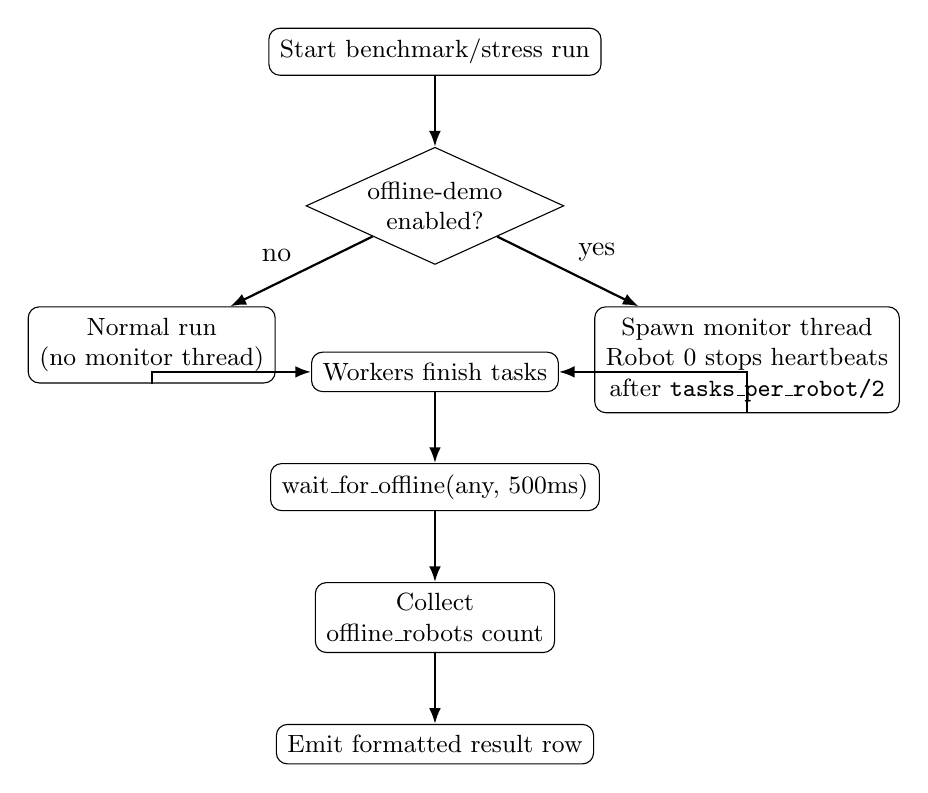
\begin{tikzpicture}[
  node distance=9mm and 12mm,
  box/.style={draw, rounded corners, align=center, inner sep=4pt, font=\small},
  decision/.style={draw, diamond, aspect=2.2, align=center, inner sep=1pt, font=\small},
  arr/.style={-{Latex[length=2mm]}, thick}
]
  \node[box] (a) {Start benchmark/stress run};
  \node[decision, below=of a] (b) {offline-demo\\enabled?};
  \node[box, below left=of b] (c) {Normal run\\(no monitor thread)};
  \node[box, below right=of b] (d) {Spawn monitor thread\\Robot 0 stops heartbeats\\after \texttt{tasks\_per\_robot/2}};
  \node[box, below=11mm of b] (e) {Workers finish tasks};
  \node[box, below=of e] (f) {wait\_for\_offline(any, 500ms)};
  \node[box, below=of f] (g) {Collect\\offline\_robots count};
  \node[box, below=of g] (h) {Emit formatted result row};

  \draw[arr] (a) -- (b);
  \draw[arr] (b) -- node[above left]{no} (c);
  \draw[arr] (b) -- node[above right]{yes} (d);
  \draw[arr] (c) |- (e);
  \draw[arr] (d) |- (e);
  \draw[arr] (e) -- (f);
  \draw[arr] (f) -- (g);
  \draw[arr] (g) -- (h);
\end{tikzpicture}
\caption{Benchmark/stress offline mode semantics aligned with the current implementation.}
\label{fig:bench-offline-flow}
\end{figure}

\subsection{Benchmark results (multi-shot summary)}
The tables below summarize three release-mode runs per configuration (mean \(\pm\) standard deviation). The selected configurations show baseline contention (4 robots, 2 zones), heavier contention (8 robots, 2 zones), improved parallelism from additional zones (8 robots, 4 zones), and offline-demo overhead on the baseline case.

\begin{table}[H]
\centering
\small
\setlength{\tabcolsep}{6pt}
\begin{tabular}{rrrrrrrr}
\toprule
Robots & Tasks/robot & Zones & Work (ms) & Offline & Elapsed (ms) & Throughput & Avg wait (\(\mu\)s) \\
\midrule
4 & 25 & 2 & 5 & no  & 309.67 \(\pm\) 8.62  & 323.10 \(\pm\) 8.93  & 4185.04 \(\pm\) 1097.86 \\
8 & 25 & 2 & 5 & no  & 620.33 \(\pm\) 12.74 & 322.50 \(\pm\) 6.55  & 11874.51 \(\pm\) 2030.96 \\
8 & 25 & 4 & 5 & no  & 326.33 \(\pm\) 11.72 & 613.41 \(\pm\) 22.44 & 5225.34 \(\pm\) 166.13 \\
4 & 25 & 2 & 5 & yes & 689.00 \(\pm\) 55.46 & 145.80 \(\pm\) 12.31 & 4514.37 \(\pm\) 627.11 \\
\bottomrule
\end{tabular}
\caption{Benchmark performance metrics (mean \(\pm\) stdev over three runs).}
\label{tab:bench-samples}
\end{table}

\begin{table}[H]
\centering
\small
\setlength{\tabcolsep}{6pt}
\begin{tabular}{rrrrrrr}
\toprule
Robots & Zones & Offline & CPU user (s) & CPU sys (s) & Max occ. & Offline robots \\
\midrule
4 & 2 & no  & 0.0005 \(\pm\) 0.0001 & 0.0018 \(\pm\) 0.0002 & 2 & 0.00 \\
8 & 2 & no  & 0.0010 \(\pm\) 0.0000 & 0.0034 \(\pm\) 0.0001 & 2 & 0.00 \\
8 & 4 & no  & 0.0010 \(\pm\) 0.0001 & 0.0049 \(\pm\) 0.0002 & 4 & 0.00 \\
4 & 2 & yes & 0.0007 \(\pm\) 0.0000 & 0.0027 \(\pm\) 0.0002 & 2 & 1.33 \(\pm\) 0.58 \\
\bottomrule
\end{tabular}
\caption{CPU and correctness summary for the same benchmark configurations (zone violations and duplicate tasks were false in all runs).}
\label{tab:bench-cpu}
\end{table}

\subsection{Scalability sweep}
Two small stress sweeps provide a quick scalability snapshot (single run per point, \texttt{work=5 ms}). The first varies robots and zones at a fixed task load; the second varies task load while holding robots and zones constant.

\begin{table}[H]
\centering
\small
\setlength{\tabcolsep}{6pt}
\begin{tabular}{rrrrrrc}
\toprule
Robots & Zones & Elapsed (ms) & Throughput & Avg wait (\(\mu\)s) & Max occ. & Zone viol. \\
\midrule
1 & 1 & 60 & 166.67 & 0.00 & 1 & false \\
1 & 2 & 57 & 175.44 & 0.00 & 1 & false \\
2 & 1 & 121 & 165.29 & 3000.55 & 1 & false \\
2 & 2 & 61 & 327.87 & 60.50 & 2 & false \\
4 & 1 & 247 & 161.94 & 9283.92 & 1 & false \\
4 & 2 & 123 & 325.20 & 3598.93 & 2 & false \\
\bottomrule
\end{tabular}
\caption{Robot/zone scalability sweep (single runs, \texttt{tasks/robot=10}).}
\label{tab:scalability}
\end{table}

\begin{table}[H]
\centering
\small
\setlength{\tabcolsep}{6pt}
\begin{tabular}{rrrrrrc}
\toprule
Robots & Tasks/robot & Zones & Elapsed (ms) & Throughput & Avg wait (\(\mu\)s) & Zone viol. \\
\midrule
4 & 10 & 2 & 123 & 325.20 & 3598.93 & false \\
4 & 25 & 2 & 308 & 324.68 & 3065.35 & false \\
4 & 50 & 2 & 616 & 324.68 & 4688.66 & false \\
\bottomrule
\end{tabular}
\caption{Task-load sweep (single runs, fixed at 4 robots and 2 zones).}
\label{tab:task-load}
\end{table}

\FloatBarrier

\subsection{Graph (throughput by robots, zones=2)}
\begin{figure}[H]
\centering
\begin{lstlisting}[language={},basicstyle=\ttfamily\small,frame=single]
Robots: 1 | ################# (175)
Robots: 2 | ################################ (328)
Robots: 4 | ############################### (325)
\end{lstlisting}
\caption{ASCII throughput visualization from a sample sweep (zones=2, robots=1,2,4).}
\label{fig:ascii-throughput}
\end{figure}

\subsection{Correctness and stress observations}
Each benchmark row summarizes three executions; short workloads are sensitive to scheduling noise, so the standard deviations provide a rough stability check. The relative trends were stable: adding robots without adding zones increased waiting time much more than it increased throughput, while adding zones restored parallelism. The offline-enabled benchmark showed a longer elapsed time because the harness waits for the timeout window to elapse before terminating the monitor thread.

\begin{itemize}[leftmargin=*]
  \item \textbf{Task safety:} No duplicate tasks were observed in any run; the validation flag remained false. This matches the queue's unit tests and indicates correct single-consumer behavior.
  \item \textbf{Zone exclusivity:} No zone violations were observed; per-zone occupancy counters never exceeded one, and max occupancy never exceeded the zone count.
  \item \textbf{Offline detection:} In deterministic demo mode, the fixed target robot is detected offline. In benchmark/stress offline mode, the final value is interpreted as \texttt{offline\_robots >= 1} because multiple robots may exceed timeout near run end.
\end{itemize}

Overall, throughput scales more strongly with additional zones than with additional robots alone. Moving from 8 robots / 2 zones to 8 robots / 4 zones raised mean throughput from 322.50 to 613.41 tasks/s while cutting average zone wait from 11874.51 to 5225.34 \(\mu\)s. The task-load sweep shows that with 4 robots and 2 zones fixed, throughput stays in a narrow 325 tasks/s band as \texttt{tasks/robot} increases from 10 to 50, while elapsed time grows roughly linearly with total work. This indicates that the optimized implementation has reduced some fixed benchmark overhead and that contention, not startup cost, is now the dominant limiter.

To further contextualize the numbers, the robot/zone sweep shows that doubling zones from 1 to 2 roughly doubled throughput at 2 robots (165.29 to 327.87 tasks/s) and similarly improved the 4-robot case (161.94 to 325.20 tasks/s), reflecting reduced blocking. The task-load sweep complements this by showing that longer runs do not introduce duplicate-task or zone-safety failures, even as total work increases. These observations align with the expected behavior of a mutex-protected resource manager: contention is the primary driver of queueing delay, adding independent resources restores parallelism, and larger workloads mostly expose steady-state coordination costs rather than correctness failures.

\section{Discussion}
The core goal of the project is correctness in concurrency, and the implementation meets this requirement by applying straightforward synchronization patterns. The task queue demonstrates a classic producer-consumer solution with a mutex and condition variable, yielding deterministic, single-consumer behavior. The zone controller models exclusive resource ownership, ensuring that a robot must explicitly acquire and release a zone, a pattern familiar from lock managers in systems and databases. The health monitor illustrates a watchdog-style approach to liveness detection and shows how timeout-driven logic can be implemented safely with a single mutex-protected state for heartbeat timestamps and offline markers.

The results highlight predictable trade-offs. When the number of robots increases without a matching increase in zones, throughput improvements are limited by contention and by the time each robot holds a zone. This is visible in the higher average zone wait times for configurations with many robots and few zones. Conversely, adding zones improves throughput and reduces wait time, demonstrating that the synchronization scheme allows parallelism when resources are available. CPU usage remains low in these microbenchmarks because most of the wall time is spent sleeping to simulate work, which is appropriate for a coordination-focused simulation.

The benchmark instrumentation confirms that per-zone occupancy never exceeded one in the sampled runs, which is consistent with the \texttt{ZoneAccess} unit tests and with the single-lock acquisition logic. This provides direct empirical evidence that the synchronization design preserves mutual exclusion under contention.

Another trade-off involves the heartbeat timeout. A shorter timeout improves detection speed but risks marking a slow robot offline. The demo uses short timeouts to make the offline event visible, whereas a real deployment would choose a longer threshold and possibly incorporate adaptive timing. The current design keeps this parameter explicit and configurable at the simulation level, which makes the timing assumptions transparent and easier to justify in a report.

From a software engineering perspective, Rust's ownership model and standard synchronization primitives promote safe concurrency. The use of \texttt{Arc} for shared ownership together with \texttt{Mutex} and \texttt{Condvar} avoids data races without requiring unsafe code. The design avoids inconsistent lock ordering, which eliminates deadlock cycles and keeps critical sections short. Recent internal optimizations preserved this simplicity: direct-indexed zone ownership, a single-lock health monitor, and a lower-overhead validation path improved benchmark behavior without introducing feature creep. This aligns with the project's decision rule of correctness over performance and supports the learning outcome that synchronization should be explicit and simple when possible.

A limitation of the current evaluation is that benchmarks are short and focused on synchronization behavior rather than sustained load. Longer runs would reduce noise in throughput and CPU measurements, and repeated trials would allow confidence intervals. Additionally, the simulation uses a fixed work duration and deterministic task-to-zone mapping, which simplifies analysis but does not capture heterogeneous task costs or dynamic zone selection. These constraints are acceptable for the minimal scope but should be revisited if the system evolves toward more realistic scheduling. From a dependability perspective, the current evaluation focuses on safety and correctness rather than on formal reliability or availability metrics \citep{avizienis2004}.

Overall, the project demonstrates that minimal, well-structured synchronization can produce a correct and observable coordination layer. The system's behavior is easy to reason about, and the design choices map cleanly to OS concurrency principles. The remaining gaps are primarily in the rigor of benchmark instrumentation and in the breadth of performance evaluation, rather than in the correctness of the core synchronization mechanisms.

\section{Conclusion and Future Work}
MCRoCS achieves its goal of implementing a lightweight OS core that safely coordinates multiple robot threads. It delivers the required task queue, zone access control, and health monitor with clear synchronization boundaries and minimal shared state. The demo shows multiple robots fetching tasks concurrently, exclusive zone occupancy, and an offline robot detected through heartbeat timeouts. Unit tests and integration tests provide direct evidence of correctness for each required component, and benchmark runs quantify throughput and waiting behavior under contention.

The project's minimal design was a deliberate choice to prioritize correctness and clarity. Using mutexes and condition variables makes the concurrency model explicit and easy to analyze, while avoiding deadlock and complex scheduling policies. The architecture is modular, with each component encapsulating its own synchronization, which simplifies reasoning and supports extension. These properties align with the learning outcomes for concurrency control, synchronization, and coordination.

Future work can build on this foundation in several directions. First, longer and repeated performance runs should be added to reduce measurement noise and to generate statistically meaningful metrics and graphs. Second, the simulation could incorporate heterogeneous task durations, dynamic zone selection, and injected delays to model more realistic operational conditions. Third, the health monitor could be extended with adaptive timeout policies or a suspicion window to balance detection speed with false-positive avoidance. Finally, if the project scope expands, it would be natural to explore advanced scheduling strategies or more scalable queue designs, while preserving the correctness guarantees that the minimal system already demonstrates.

To improve evaluation quality further, benchmark and stress modes could adopt deterministic liveness attribution similar to the demo rather than relying only on ``any offline'' outcomes. In practical terms, a fixed target robot could be selected to stop heartbeats while non-target robots continue sending periodic heartbeats until timeout verification finishes. That extension would make workload-timeout results easier to interpret, because the summary could distinguish the intended offline robot from incidental end-of-run silence.

In its current form, the system is already suitable for the required demo and report deliverables: it has a clear architecture, observable concurrency behavior, and a clean test suite that verifies the three mandatory components. These qualities make it a strong baseline for any future extensions.

\begin{thebibliography}{99}
\bibitem[Arpaci-Dusseau \& Arpaci-Dusseau(2023)]{arpaci2018} Arpaci-Dusseau, R. H., \& Arpaci-Dusseau, A. C. (2023). \textit{Operating Systems: Three Easy Pieces} (Version 1.10). Arpaci-Dusseau Books. Retrieved February 2, 2026, from https://pages.cs.wisc.edu/~remzi/OSTEP/
\bibitem[Birrell(1989)]{birrell1989} Birrell, A. D. (1989). \textit{An Introduction to Programming with Threads}. Digital Equipment Corporation.
\bibitem[Dijkstra(n.d.)]{dijkstra1965} Dijkstra, E. W. (n.d.). \textit{Cooperating sequential processes (EWD 123)}. Retrieved February 2, 2026, from https://www.cs.utexas.edu/~EWD/transcriptions/EWD01xx/EWD123.html
\bibitem[Downey(2016)]{downey2016} Downey, A. B. (2016). \textit{The Little Book of Semaphores} (2nd ed.). Green Tea Press.
\bibitem[Hoare(1974)]{hoare1974} Hoare, C. A. R. (1974). Monitors: An operating system structuring concept. \textit{Communications of the ACM, 17}(10), 549--557.
\bibitem[Lampson \& Redell(1980)]{lampson1980} Lampson, B. W., \& Redell, D. D. (1980). Experience with processes and monitors in Mesa. \textit{Communications of the ACM, 23}(2), 105--117.
\bibitem[Lamport(1978)]{lamport1978} Lamport, L. (1978). Time, clocks, and the ordering of events in a distributed system. \textit{Communications of the ACM, 21}(7), 558--565.
\bibitem[Herlihy et~al.(2020)]{herlihy2020} Herlihy, M., Shavit, N., Luchangco, V., \& Spear, M. (2020). \textit{The Art of Multiprocessor Programming} (2nd ed.). Morgan Kaufmann.
\bibitem[Silberschatz et~al.(2018)]{silberschatz2018} Silberschatz, A., Galvin, P. B., \& Gagne, G. (2018). \textit{Operating System Concepts} (10th ed.). Wiley.
\bibitem[Tanenbaum \& Bos(2015)]{tanenbaum2015} Tanenbaum, A. S., \& Bos, H. (2015). \textit{Modern Operating Systems} (4th ed.). Pearson.
\bibitem[Williams(2019)]{williams2019} Williams, A. (2019). \textit{C++ Concurrency in Action} (2nd ed.). Manning.
\bibitem[Klabnik \& Nichols(2022)]{klabnik2022} Klabnik, S., \& Nichols, C. (2022). \textit{The Rust Programming Language} (2nd ed.). No Starch Press.
\bibitem[Rust Project(n.d.-a)]{rustmutex} Rust Project. (n.d.). \textit{std::sync::Mutex}. Retrieved February 2, 2026, from https://doc.rust-lang.org/std/sync/struct.Mutex.html
\bibitem[Rust Project(n.d.-b)]{rustcondvar} Rust Project. (n.d.). \textit{std::sync::Condvar}. Retrieved February 2, 2026, from https://doc.rust-lang.org/std/sync/struct.Condvar.html
\bibitem[Rust Project(n.d.-c)]{rustarc} Rust Project. (n.d.). \textit{std::sync::Arc}. Retrieved February 2, 2026, from https://doc.rust-lang.org/std/sync/struct.Arc.html
\bibitem[Rust Project(n.d.-e)]{rustinstant} Rust Project. (n.d.). \textit{std::time::Instant}. Retrieved February 2, 2026, from https://doc.rust-lang.org/std/time/struct.Instant.html
\bibitem[Gray \& Reuter(1993)]{gray1993} Gray, J., \& Reuter, A. (1993). \textit{Transaction Processing: Concepts and Techniques}. Morgan Kaufmann.
\bibitem[Lynch(1996)]{lynch1996} Lynch, N. (1996). \textit{Distributed Algorithms}. Morgan Kaufmann.
\bibitem[Chandra \& Toueg(1996)]{chandra1996} Chandra, T. D., \& Toueg, S. (1996). Unreliable failure detectors for reliable distributed systems. \textit{Journal of the ACM, 43}(2), 225--267.
\bibitem[Avizienis et~al.(2004)]{avizienis2004} Avizienis, A., Laprie, J.-C., Randell, B., \& Landwehr, C. (2004). \textit{Basic concepts and taxonomy of dependable and secure computing} (Technical Report No. UMIACS-TR-2004-47). University of Maryland, Institute for Systems Research. Retrieved February 2, 2026, from https://drum.lib.umd.edu/items/6b297ffc-373b-404f-be3a-70cc849e21fd
\end{thebibliography}

\end{document}
